\chapter{Estado del Arte}
Para fundamentar la solución propuesta en esta tesis, resulta imprescindible analizar el 
panorama actual de las herramientas digitales y los modelos computacionales aplicados al 
diagnóstico dermatológico. El presente capítulo aborda, en primer lugar, una revisión de 
plataformas comerciales ampliamente utilizadas a nivel internacional, como DermEngine, 
SkinVision y VisualDx, evaluando sus características funcionales, costos de acceso y 
limitaciones para su implementación en el contexto cubano. En segundo lugar, se examinan 
sistemas académicos de referencia, incluyendo el archivo ISIC (International Skin 
Imaging Collaboration) y el conjunto de datos HAM10000, así como los modelos de 
aprendizaje automático derivados de ellos. A continuación, se describen las técnicas 
más relevantes de aprendizaje de máquinas en dermatología, el aprendizaje por transferencia y los enfoques de 
inteligencia artificial explicable (XAI), estos últimos particularmente importantes 
dotar al sistema de un modelo que justifique sus diagnósticos. 
Finalmente, se identifica una brecha clara entre las soluciones existentes y los 
requerimientos específicos que debe cumplir DermaUH, lo que justifica el desarrollo 
de una nueva versión adaptada a las condiciones de conectividad, disponibilidad de datos 
y necesidades de los dermatólogos cubanos.

\section{Herramientas existentes}

En esta sección se realizará un análisis de algunas de las aplicaciones que se utilizan
para brindar ayuda en los diagnósticos dermatológicos. Dicho análisis se efectuará
atendiendo a sus funcionalidades principales, ventajas y desventajas para el contexto cubano de 
cada aplicación móvil o web.

\subsection*{Criterios de selección}
Para la selección de las herramientas analizadas en profundidad, se establecieron los siguientes 
criterios de inclusión: (1) disponibilidad comercial o acceso público desde al menos 2020,
año a partir del cual se generalizó el uso de redes neuronales convolucionales en dermatología; 
(2) uso explícito de inteligencia artificial (preferentemente redes neuronales convolucionales) 
para la clasificación o análisis de lesiones cutáneas; (3) presencia de estudios clínicos 
publicados o certificaciones regulatorias (como marcado CE o aprobación de la FDA); 
(4) representatividad de diferentes modelos de negocio (suscripción, pago por uso, etc.). 
Con base en estos criterios, se seleccionaron tres herramientas: \textbf{DermEngine}, 
\textbf{SkinVision} y \textbf{VisualDx}. 

Existen otras aplicaciones como Miiskin o First Derm, pero quedaron excluidas por no cumplir 
con el criterio (3) al carecer de estudios clínicos publicados que respalden su eficacia 
diagnóstica en el contexto dermatológico, o por estar orientadas exclusivamente a la 
teleconsulta sin componente de IA propio.

Las herramientas escogidas tienen en común el uso de modelos de aprendizaje automático como 
principal engranaje para asistir en los diagnósticos. Además, cada una cuenta con su propia 
base de imágenes, lo que permite un análisis comparativo de este aspecto tan importante, 
el cual forma parte del objetivo principal de esta tesis.

\subsection{DermEngine}
\begin{figure}[ht] 
    \centering
    
\includegraphics[width=0.3\textwidth]{Graphics/dermengine_logo.png}
    \caption{Logo de DermEngine} 
    \label{logoDermEngine}
\end{figure}

\href{https://www.dermengine.com/es/}{DermEngine}\cite{dermEngine} es una plataforma de software 
inteligente diseñada específicamente para dermatología, cuyo principal objetivo es 
optimizar el flujo de trabajo clínico mediante la integración de inteligencia 
artificial en el análisis de imágenes dermatoscópicas. Entre sus funcionalidades más 
relevantes se encuentran (estudio realizado en Marzo del 2026):
\begin{enumerate}
    \item \textbf{Búsqueda visual inteligente (Visual Search)}: Utiliza un algoritmo de inteligencia artificial que compara una imagen de una lesión con una base de datos de miles de casos etiquetados. A partir de esta comparación, el sistema genera una lista de posibles diagnósticos y ofrece una estimación del riesgo de malignidad, actuando como una segunda opinión automatizada para el especialista.
    \item \textbf{Gestión integral de pacientes y lesiones}: Permite registrar y organizar la información clínica de los pacientes, incluyendo imágenes de sus lesiones, historiales de seguimiento y notas clínicas.
    \item \textbf{Integración con dispositivos de captura}: Se conecta con MoleScope, un dermatoscopio digital de bajo costo que se acopla a teléfonos inteligentes.
    \item \textbf{Imagenología de cuerpo completo}: Ofrece herramientas para mapear la superficie corporal del paciente y documentar la ubicación exacta de cada lesión.
    \item \textbf{Colaboración y teledermatología}: Permite compartir casos entre especialistas de manera segura, obtener segundas opiniones y realizar sesiones de teleconsulta.
\end{enumerate}

\subsubsection{Ventajas}
\begin{enumerate}
    \item \textbf{Optimización del diagnóstico}: La IA proporciona una referencia rápida que puede aumentar la confianza del especialista.
    \item \textbf{Herramienta educativa}: La base de datos de imágenes etiquetadas puede utilizarse para la formación de residentes y estudiantes.
    \item \textbf{Seguimiento longitudinal}: La comparación de imágenes a lo largo del tiempo es crucial para la detección precoz de melanomas.
    \item \textbf{Posible integración con dispositivos móviles}: Compatibilidad con MoleScope para captura estandarizada.
\end{enumerate}

\subsubsection{Desventajas}
\begin{enumerate}
    \item \textbf{Dependencia de conectividad a internet}: Plataforma basada en la nube, requiere conexión estable y rápida.
    \item \textbf{Costo de acceso}: Suscripción desde 99 USD mensuales, inaccesible para dermatólogos cubanos.
    \item \textbf{Barreras idiomáticas}: Interfaz y documentación principalmente en inglés.
    \item \textbf{Falta de adaptación a la población cubana}: Modelos entrenados mayoritariamente con pieles claras, sin validación en fototipos II-VI (pieles m\'as oscuras).
\end{enumerate}

\subsection{SkinVision}
\begin{figure}[ht] 
    \centering
    
\includegraphics[width=0.3\textwidth]{Graphics/skinvision_logo.png}
    \caption{Logo de SkinVision} 
    \label{logoSkinVision}
\end{figure}

\href{https://www.skinvision.com/}{SkinVision} es una aplicación móvil de servicio médico 
de pago, clínicamente validada, cuyo principal objetivo es la detección temprana del cáncer 
de piel enfocada en el autocuidado. Utiliza una red neuronal convolucional ResNet-50 para 
analizar imágenes de lunares o manchas cutáneas, clasificando las lesiones en riesgo alto, 
bajo o en revisión.

\begin{figure}[ht] 
    \centering
    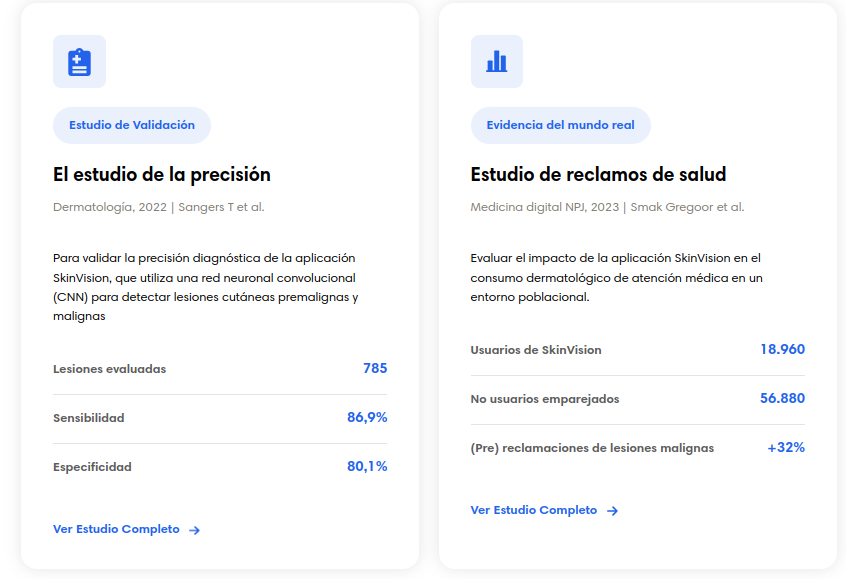
\includegraphics[width=0.8\textwidth]{Graphics/estudio_skinvision.png}
    \caption{Estudio clínico de SkinVision} 
    \label{estudioSkinVision}
\end{figure}

El proceso de evaluación consta de cuatro etapas: captura guiada de la imagen, análisis 
por IA (sensibilidad 92.1\% para melanoma, 98.6\% para carcinoma escamoso), revisión 
secundaria por expertos en casos de riesgo alto o en revisión, y entrega de resultados al usuario.

\begin{figure}[ht] 
    \centering
    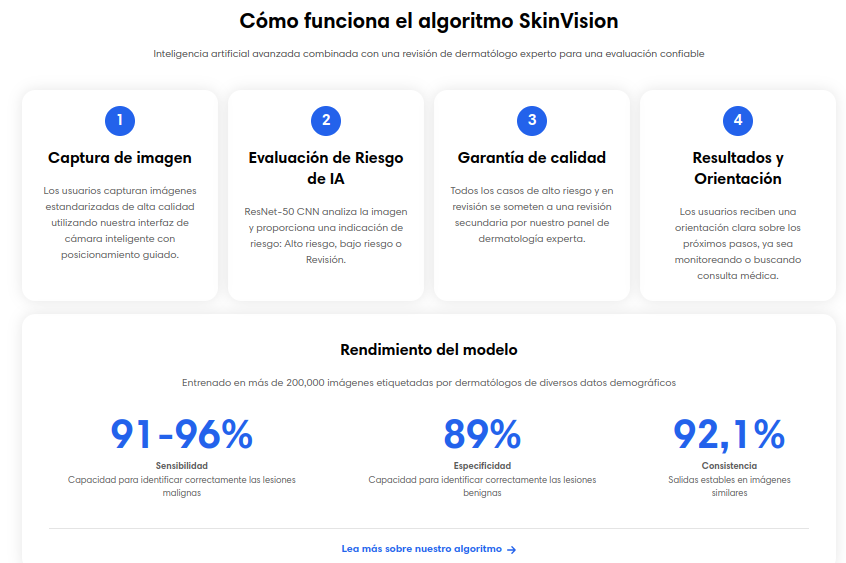
\includegraphics[width=0.8\textwidth]{Graphics/modelo_skinvision.png}
    \caption{Diagrama del algoritmo de SkinVision} 
    \label{modeloSkinVision}
\end{figure}

\subsubsection{Ventajas}
\begin{enumerate}
    \item \textbf{Alta sensibilidad diagnóstica}: Reporta hasta 95\% de sensibilidad para lesiones malignas.
    \item \textbf{Validación clínica y regulatoria}: Certificación CE como dispositivo médico Clase IIa.
    \item \textbf{Alta especificidad}: 89\% en métricas recientes, reduciendo falsas alarmas.
    \item \textbf{Revisión por expertos}: Control de calidad adicional para casos de alto riesgo.
\end{enumerate}

\subsubsection{Desventajas}
\begin{enumerate}
    \item \textbf{Enfoque en el paciente, no en el especialista}: No provee herramientas para gestión clínica.
    \item \textbf{Costo de acceso}: Plan anual de aproximadamente €49.99, inaccesible para el sistema de salud cubano.
    \item \textbf{Dependencia de conectividad}: Requiere internet para procesar imágenes en sus servidores.
    \item \textbf{Falta de adaptación a pieles cubanas}: Entrenado mayoritariamente con pieles claras europeas, riesgo de sesgo.
    \item \textbf{Potencial de falsa seguridad}: Un resultado de bajo riesgo podría retrasar una consulta médica necesaria.
\end{enumerate}

\subsection{VisualDx}
\begin{figure}[ht] 
    \centering
    
\includegraphics[width=0.3\textwidth]{Graphics/visualdx_logo.png}
    \caption{Logo de VisualDx} 
    \label{logoVisualDx}
\end{figure}

\href{https://www.visualdx.com/}{VisualDx}\cite{visualDx} es un sistema de apoyo a la decisión clínica que combina 
inteligencia artificial con una extensa biblioteca de imágenes médicas. Asiste a médicos no 
especialistas (atención primaria, urgencias) en el diagnóstico de enfermedades de la piel, 
reduciendo derivaciones a dermatología entre 25\% y 45\%.

\subsubsection{Ventajas}
\begin{enumerate}
    \item \textbf{Enfoque en atención primaria}: Útil en contextos con acceso limitado al especialista. Los usuarios podr\'an realizar consultas ``menores'' en caso de no poder asistir a la consulta del doctor.
    \item \textbf{Biblioteca inclusiva de pieles oscuras}: Ha trabajado durante 20 años en incluir fototipos II-VI.
    \item \textbf{Apoyo al diagnóstico diferencial}: Basado en síntomas y demografía del paciente.
    \item \textbf{Integración de IA y evidencia médica}: El usuario puede tomar una fotograf\'ia con su celular, no neceseriamente con el dermatoscopio. Acto seguido rellena informaci\'on sobre el paciente, como profesi\'on, exposici\'on al sol y antecedentes. La IA de VisualDx combina la imagen, con esa informaci\'on y genera un diagn\'ostico que luego ser\'a validado por el especialista.
\end{enumerate}

\subsubsection{Desventajas}
\begin{enumerate}
    \item \textbf{Costo prohibitivo}: Suscripciones entre 299.99 y 649.99 euros anuales.
    \item \textbf{Dependencia de internet}: Requiere conexión constante para acceder a la biblioteca y la IA.
    \item \textbf{No diseñada para especialistas}: Orientada a médicos generales, no a dermatólogos para su práctica diaria.
\end{enumerate}

\subsection{Conclusiones del análisis de herramientas}

En esta sección se analizaron herramientas con fines similares a DermaUH 3.0. A partir del análisis anterior, se presenta la Tabla~\ref{tab:comparativa_herramientas} con un resumen comparativo.

\begin{table}[ht]
    \centering
    \footnotesize
    \caption{Comparativa de herramientas comerciales de diagnóstico dermatológico asistido por IA}
    \label{tab:comparativa_herramientas}
    \begin{tabularx}{\textwidth}{|>{\raggedright\arraybackslash}X|>{\raggedright\arraybackslash}X|>{\raggedright\arraybackslash}X|>{\raggedright\arraybackslash}X|>{\raggedright\arraybackslash}X|>{\raggedright\arraybackslash}X|>{\raggedright\arraybackslash}X|}
        \hline
        \textbf{Herramienta} & \textbf{Tipo de IA} & \textbf{Conjunto de datos (origen / fototipos)} & \textbf{Métricas reportadas} & \textbf{Costo (anual aprox.)} & \textbf{Dependencia internet} & \textbf{Lección para DermaUH} \\
        \hline
        DermEngine & CNN (Visual Search) & Mayormente pieles claras (Europa/EE.UU.) & No especifica públicamente & \$1188 USD & Alta (nube) & Evitar dependencia total de la nube \\
        \hline
        SkinVision & ResNet-50 & Mayormente pieles claras (Europa) & Sensibilidad 95\%, Especificidad 89\% & €50 & Alta & La alta sensibilidad no es suficiente; se necesita explicabilidad \\
        \hline
        VisualDx & DermExpert (propietario) & Incluye pieles oscuras (28.5\%) pero con sesgo & Reducción derivaciones 25-45\% & \$299-649 & Alta & Inclusión de pieles oscuras es insuficiente sin validación local \\
        \hline
    \end{tabularx}
\end{table}

A partir del análisis se extraen los siguientes hechos concretos:

\begin{enumerate}
    \item \textbf{Conjunto de imágenes}: VisualDx incluye pieles oscuras, pero las m\'etricas de sus modelos son muy altas cuando debe clasificarlas; DermEngine y SkinVision usan mayoritariamente pieles claras, las pieles cubanas son en su mayor\'ia mestizas u oscuras, por tanto el hecho de tener solamente etnias claras provocar\'ia un sesgo y una bajada en las m\'etricas al analizar pieles cubanas.
    \item \textbf{Costo de suscripción}: Períodos de prueba gratuitos breves (7-30 días). Las suscripciones son inaccesibles para el sistema de salud cubano.
    \item \textbf{Modelo explicativo}: Ninguna herramienta incorpora inteligencia artificial explicable (XAI) que justifique el diagnóstico.
    \item \textbf{Rendimiento}: DermEngine incluye un video de 3 minutos en su portada; SkinVision abusa de animaciones y videos, degradando el rendimiento sin conexión rápida.
\end{enumerate}

\subsubsection*{Lecciones para DermaUH 3.0}

Del análisis anterior, DermaUH 3.0 debe adoptar las siguientes decisiones de diseño:

\begin{itemize}
    \item \textbf{Modelo entrenado con pieles cubanas}: Buscar m\'as representatividad de los fototipos del IV-VI para el conjunto de datos de entrenamiento, los cuales son los predominantes en la poblaci\'on cubana.
    \item \textbf{Explicabilidad diagnóstica}: Incorporar un modelo XAI que justifique cada predicción, aumentando la confianza del especialista.
    \item \textbf{Gratuidad total}: La plataforma será completamente gratuita para el sistema de salud cubanos, eliminando la barrera económica.
    \item \textbf{Optimización de rendimiento}: Priorizar un diseño ligero, con tiempos de carga optimizados y consumo eficiente de recursos, evitando videos o animaciones pesadas.
\end{itemize}

Estas lecciones reflejan la importancia de desarrollar una aplicación para el diagnóstico 
asistido por IA, libre de costo, con modelos entrenados con imágenes de pieles cubanas, 
que integre un modelo explicativo y que funcione adecuadamente en las condiciones de 
conectividad del sistema de salud cubano.

\section{Archivos acad\'emicos de referencia}
Además de las herramientas comerciales, es necesario estudiar los repositorios 
académicos que sirven como base para el entrenamiento de modelos de IA:

\subsection{ISIC Archive: Repositorio académico de referencia}

La \textbf{International Skin Imaging Collaboration (ISIC) Archive}\cite{isic} es un repositorio 
público de acceso abierto que contiene una de las colecciones más grandes y completas 
del mundo de imágenes dermatoscópicas y metadatos clínicos asociados. Concebido para 
apoyar la docencia, la investigación y el desarrollo de algoritmos de inteligencia 
artificial, el archivo se ha convertido en el banco de pruebas estándar para sistemas 
de diagnóstico asistido en dermatología. Las imágenes provienen de múltiples centros 
internacionales y han sido etiquetadas mediante confirmación histopatológica (el 
estándar de oro) o por consenso de múltiples expertos, lo que garantiza un alto grado 
de fiabilidad diagnóstica. Su impacto trasciende lo puramente científico, pues las 
competiciones anuales conocidas como \textit{ISIC Challenges} han permitido a la 
comunidad de ciencia de la computación contribuir activamente a la mejora de estos 
sistemas, moviendo los límites del rendimiento de los modelos de aprendizaje automático.

\subsubsection{Organización de los datos}

Los datos de la ISIC Archive están organizados siguiendo una jerarquía de categorías 
y marcos taxonómicos que facilitan el desarrollo de modelos de inteligencia artificial. 
Las Tablas~\ref{tab:isic_categorias} y~\ref{tab:isic_atributos} detallan las principales 
vías de clasificación dentro del ecosistema: un marco general de clasificación por 
diagnóstico (utilizado tanto por los médicos como por el dataset HAM10000 integrante 
del archivo) y un marco orientado al desarrollo de algoritmos de \textit{machine learning}, 
que incorpora la atribución de diagnóstico para problemas multiclase.

\begin{table}[ht]
    \centering
    \caption{Principales categorías generales de diagnóstico de lesiones en el archivo ISIC y el dataset HAM10000}
    \label{tab:isic_categorias}
    \begin{tabularx}{\textwidth}{|>{\raggedright\arraybackslash}X|>{\raggedright\arraybackslash}X|>{\raggedright\arraybackslash}X|}
        \hline
        \textbf{Categoría General} & \textbf{Descripción} & \textbf{Ejemplos de Subcategorías} \\
        \hline
        Lesiones Melanocíticas & Lesiones pigmentadas originadas de melanocitos. & Nevo Melanocítico (Benigno), Melanoma (Maligno) \\
        \hline
        Lesiones Queratinocíticas & Lesiones derivadas de células queratinizantes. & Queratosis Actínica / Enfermedad de Bowen, Queratosis Benignas (queratosis seborreica) \\
        \hline
        Neoplasias Vasculares / Raras & Lesiones con origen en vasos sanguíneos o de presentación poco común. & Lesiones Vasculares, Dermatofibroma \\
        \hline
        Carcinoma de Células Basales (BCC) & Tumor maligno de células basales, el más común. & Carcinoma Basocelular (BCC) \\
        \hline
    \end{tabularx}
    \small{\textit{Nota:} El número de clases presentadas y su agrupación puede variar ligeramente entre las diferentes versiones del dataset (por ejemplo, 2018, 2019).}
\end{table}

\begin{table}[ht]
    \centering
    \caption{Metadatos asociados a los diagnósticos y marco de tareas para la comunidad de Machine Learning}
    \label{tab:isic_atributos}
    \begin{tabularx}{\textwidth}{|>{\raggedright\arraybackslash}p{3.2cm}|>{\raggedright\arraybackslash}p{2.8cm}|>{\raggedright\arraybackslash}X|}
        \hline
        \textbf{Caso de Uso / Metadato} & \textbf{Nivel Jerárquico} & \textbf{Atributos y Descripción} \\
        \hline
        Atributos de Diagnóstico de Alto Nivel & Diagnóstico de Lesión & \textbf{Benigna:} Nevo Melanocítico, Queratosis Benigna, Dermatofibroma. \\
        & & \textbf{Indeterminada/Pre-Maligna:} Queratosis Actínica / Enfermedad de Bowen. \\
        & & \textbf{Maligna:} Melanoma, Carcinoma Basocelular (BCC). \\
        \hline
        Diagnóstico Específico & Lesión Específica & Permite clasificaciones de hasta quinto nivel, identificando patologías concretas según la taxonomía ISIC-IDDX. \\
        \hline
        Confirmación del Diagnóstico (\texttt{diagnosis confirm type}) & Mecanismo de Verificación & Identifica si la etiqueta se obtuvo por \textbf{confirmación histopatológica} o por \textbf{consenso de expertos}. \\
        \hline
        Subtareas de la Competencia ISIC & Problema de ML & \textbf{Segmentación:} Delimitación de los bordes de la lesión. \\
        & & \textbf{Detección de Atributos Dermoscópicos} (ATZ). \\
        & & \textbf{Clasificación:} Distinción entre lesiones benignas y malignas. \\
        \hline
    \end{tabularx}
    \small{\textit{Nota:} \texttt{diagnosis\_confirm\_type} ``histopathology'' se refiere a la confirmación mediante biopsia o análisis de tejido; ``consensus'' implica un acuerdo diagnóstico entre múltiples dermatólogos expertos sin necesidad de biopsia.}
\end{table}

Este andamiaje de datos, etiquetas y desafíos competitivos ha posicionado a la ISIC Archive 
como el estándar de facto para la comparación de algoritmos, impulsando el progreso en la 
detección automatizada del melanoma a nivel mundial. Adem\'as de eso existen numerosos conjuntos
de datos (Datasets), derivados de ISIC, que han sido utilizados en art\'iculos cient\'ificos,
proyectos de ML e investigaciones relacionadas con la IA. A continuaci\'on una menci\'on y breve
explicaci\'on de algunos de estos datasets.

\subsection{DERM12345}
Seg\'un un art\'iculo presentado por la revista Nature (una de las más prestigiosas revistas 
científicas a nivel mundial, fundada por el astrónomo británico Joseph Norman Lockyer.),
presenta un conjunto de datos diversos que comprende 12.345 imágenes dermatoscópicas 
con 40 subclases de lesiones cutáneas, recogidas en Turkiye, que comprende diferentes 
tipos de piel en la zona de transición entre Europa y Asia. Cada subgrupo contiene 
imágenes de alta resolución y anotaciones de expertos, proporcionando una base sólida y 
confiable para futuras investigaciones. El análisis detallado de cada subgrupo 
proporcionado en este estudio facilita los esfuerzos de investigación dirigidos y 
mejora la profundidad de la comprensión con respecto a las lesiones de la piel. 
Este conjunto de datos se distingue a través de una estructura diversa con sus 5 súper 
clases, 15 clases principales, 40 subclases y 12.345 imágenes dermatoscópicas de alta 
resolución\cite{Derm12345}.

\subsection{HAM10000}
Otro art\'iculo presentado en la revista Natura, referido al dataset HAM10000 expresa que
el conjunto de datos final consta de 10015 imágenes dermatoscópicas que se publican como 
un conjunto de capacitación para fines académicos de aprendizaje automático y están 
disponibles públicamente a través del archivo de la ISIC. Este conjunto de datos de 
referencia se puede utilizar para el aprendizaje automático y para comparaciones con 
expertos humanos. Los casos incluyen una colección representativa de todas las categorías 
de diagnóstico importantes en el ámbito de las lesiones pigmentadas. Más del $50\%$ 
de las lesiones han sido confirmadas por patología, mientras que la verdad fundamental 
para el resto de los casos fue el seguimiento, el consenso de expertos o la confirmación 
por microscopía confocal en vivo\cite{HAM1000}.

\subsection{Conclusiones parciales sobre los archivos acad\'emicos de referencia}
Aunque estos dataset son altamente reconocidos y utilizados en dis\'imiles de aplicaciones
a nivel mundial, no cumplen con los requisitos del conjunto de datos necesitados en la versi\'on 3.0
de DermaUH. Por ejemplo el conjunto de datos DERM12345, recopil\'o informaci\'on mayormente
en Turkye, espec\'ificamente la zona de transici\'on entre Europa y Asia en las cuales 
existen factores externos que pueden provocar en las lesiones cut\'aneas registradas un 
comportamiento y evoluci\'on diferente al esperado en pieles cubanas, 
dichos factores pueden ser intensidad del sol en esta parte del planeta, 
el clima y las temperaturas\cite{pielClima}. Por otro lado el dataset HAM10000, est\'a 
conformado por un alto n\'umero de pieles claras, provocando que los modelos ML 
que se pueden entrenar tengan un alto sesgo de este tipo de piel.

\section{Técnicas de inteligencia artificial explicable XAI en dermatología}
Seg\'un la tesis de la Licenciada Amanda Noris\cite{tesisAmanda}, la inteligencia artificial
explicativa (XAI) surge como respuesta al creciente uso de modelos de IA cuyos procesos de toma
desiciones son dif\'iciles de interpretar. Los m\'etodos XAI se dividen en dos grandes enfoques:
\begin{itemize}
    \item Modelos intr\'insicamente explicables: Buscan dise\~nar modelos cuya estructura sea comprensible por si misma. 
    \item T\'ecnicas de explicaci\'on post-hoc: Interpretan modelos ya entrenados.
\end{itemize}